Let us take the first step of our journey towards high-performance computing on
GPUs with a low-performance simple program that does hardly no computing. We
will modify a typical ``Hello, World!'' program in C++ slightly by adding a few
more lines (marked below with the comment \texttt{/* UAMMD */}). Note that we
also included the \texttt{using std::make\_shared} line so that we can later
declare \texttt{System} as a shared pointer (if you do not know what this means,
it doesn't matter right now).
\begin{lstlisting}
%! codefile: code/minimal.cu
# include <iostream>
# include "uammd.cuh" /* UAMMD */

using namespace uammd; /* UAMMD */
using std::make_shared;
using std::endl;
using std::cout;

int main(int argc, char *argv[]){

  auto sys = make_shared<System>(argc,argv); /* UAMMD */

  cout<<endl<<"--> Hello, UAMMD! <--"<<endl<<endl;

  sys->finish(); /* UAMMD */

  return 0;
}
%! codeend
\end{lstlisting}
Compile the code with
\begin{verbatim}
nvcc -O3 -I../uammd/src -I../uammd/src/third_party -o minimal
minimal.cu
\end{verbatim}
making sure that you replace the paths to UAMMD src code with the right path on
your system. With luck, the program will compile without problems. If it does
not, check the instructions for your system and the compiling information at the
UAMMD repository.

Running \texttt{./minimal} outputs some UAMMD information, with your ``Hello, 
UAMMD!'' message in the middle. Take out all the lines marked \texttt{/* UAMMD 
*/} and you are left with a typical ``Hello, World!'' program in C++ that only 
outputs your message.

It might be helpful to go through the program to explain what each UAMMD line 
does in very general terms. You \texttt{include} the \texttt{uammd.cuh} header 
file and use the \texttt{uammd} namespace to have access to the functionality 
defined in the UAMMD source code. Within the main function, we enclose all our 
UAMMD code between the creation of a \texttt{System} and its \texttt{finish}
call. The \texttt{System} represents the computing environment in UAMMD. It
deals with access to the GPU and random number generation on the CPU, for
example. In the code above, we created a \texttt{System} named \texttt{sys} with
\begin{verbatim}
auto sys = make_shared<System>(argc,argv);
\end{verbatim}
and called \texttt{sys->finish()} at the end of the program to ensure a graceful
exit.

The program compiles and runs, but it feels like an empty sandwich. By expanding
it slightly, though, we can run a simple simulation.

\section{\label{physical_system}The physical system}

The main sandwich filling in our virtual kitchen has to be the physical system
that we wish to simulate, represented as a collection of particles. Define them
with the following lines after declaring \texttt{sys}.
\begin{lstlisting}
%! codeblock: particleData
  int numberOfParticles = 100000;
  auto particles
    = make_shared<ParticleData>(numberOfParticles, sys);
%! codeblockend
\end{lstlisting}
From now on, we have access to all the properties of our particles. We might, 
for example, decide to distribute the particles randomly within an imaginary 
128-unit box. In the following snippet, a code block set apart by brackets
defines \texttt{position} as a local variable, meaning that it cannot be
accessed from  other parts of the code, in contrast to \texttt{L}. Let it
replace the ``Hello, UAMMD!'' line above.\label{initialConditions}
\begin{lstlisting}
%! codeblock: initialConditions
  real L = 128;
  %! codeinsert: simulationBox

  {
    auto position
      = particles->getPos(access::location::cpu,
                          access::mode::write);

    for(int i = 0; i < numberOfParticles; ++i)
      position[i]
        = make_real4(sys->rng().uniform3(-0.5, 0.5), 0)*L;
  }
%! codeblockend
\end{lstlisting}
In the \texttt{for} loop we go over the list of positions and assign to each of
them a random four-dimensional vector. The first three components are random
numbers chosen from a uniform distribution between $-0.5$ and $0.5$ the last one
is zero. Because we then multiply the vector by \texttt{L}, we finally get
coordinates in the $-\frac{L}{2}$ to $\frac{L}{2}$ range. \texttt{L} was defined
as a \texttt{real} value. Depending on the options at compilation, this means
either a floating point or a double precision number. The final number in the
four-vector represents the particle type (here set to zero).

Making the position variable local guarantees that we will not try to read it
later on, thinking that we have access to the positions, but without having
received the updated values. Use \texttt{getPos} every time you need to access
the positions.

Suppose that, instead of writing to the particle positions, we wished to read
the velocities. The code snippet would resemble the box above, but we would call
\texttt{getVel} instead of \texttt{getPos} and indicate that we wish to read the
values.
\begin{lstlisting}
    auto velocities
      = particles->getVel(access::location::cpu,
                          access::mode::write);
%!
\end{lstlisting}
Other particle properties work similarly: use \texttt{getMass},
\texttt{getRadius}, \texttt{getCharge}, \texttt{getForce} or \texttt{getEnergy}.

Each particle is born with a name or identification number, which you may think
of as a serial number, accessible with the \texttt{getId} method. The reason why
you should care about this name concerns UAMMD reshuffling all the particles
every once in a while for efficiency. If you wish to track the trajectory of the
particle pointed at by \texttt{positions[3]}, you must remember that later on in
the code, when you get the positions with \texttt{getPos}, \texttt{positions[3]}
might be pointing at the location of a different particle.

Generally speaking, you will want to traverse the particle data in the order
provided by these \texttt{getWhatever} functions when you want to perform an
operation on all the particles, but don't care about the order, like when you
calculate the force on each particle. If you wish to track trajectories, for
example, then you need to identify the particles by name. So, if you would
like to print out the positions in the same order every time, use this:
\label{particlePositions}
\begin{lstlisting}
      auto position
        = particles->getPos(access::location::cpu,
                            access::mode::read);
      const int * index = particles->getIdOrderedIndices(access::location::cpu);

      out<<endl;
      for(int id = 0; id < numberOfParticles; ++id)
        out<<position[index[id]]<<endl;
%!
\end{lstlisting}
After getting the positions, you get a list of the indices ordered by name. Say
that you are searching for a particle with \texttt{id = 3}. Then
\texttt{index[id]} would tell you where it lies in the particle list, and
\texttt{position[index[id]]} would give you its position in space (and its type
as the fourth component of the position vector).

\section{Integrating the equations of motion}

The next ingredients adding flavour to our sandwich are time and motion. To get
the particles to move, we have to integrate their equations of motion
numerically. Now, we keep the new feature as simple as possible by assuming that
the particles do not interact, and treat them as atoms in an ideal gas.

We need some more functionality, which we import into our project with
\begin{lstlisting}
# include "Integrator/VerletNVE.cuh"
%!
\end{lstlisting}
at the beginning of the file, after including the \texttt{uammd.cuh} header 
file. Now we can use the Verlet scheme to integrate the equations of motion, but 
we need to set the values of some parameters first. \texttt{dt} sets the size of 
the integration time step. In the introduction, we used Euler's algorithm to 
carry out the integration, but Verlet came up with a very popular method which 
improved the accuracy of integration at very little extra computational cost.
\begin{lstlisting}
%! codeblock: VerletParams
  using Verlet = VerletNVE::VerletNVE;
  Verlet::Parameters VerletParams;
  VerletParams.dt = 0.01;
  VerletParams.initVelocities=true;
  VerletParams.energy = 1.0;
%! codeblockend
\end{lstlisting}
In addition, we use the algorithm to initialise the velocities to random values
in such a way that the energy per particle equals \texttt{1.0}. Having set the
parameters, we activate the integrator with the following line.
\begin{lstlisting}
%! codeblock: Verlet
  auto integrator
    = make_shared<Verlet>(particles, sys, VerletParams);
%! codeblockend
\end{lstlisting}

Leaving their initial random positions, we allow the atoms to drift away. The 
program, we decide, will write the positions to \texttt{free\_expansion.dat}.
\begin{lstlisting}
%! codeblock: outputFile
  std::string outputFile = "free_expansion.dat";
  std::ofstream out(outputFile);

  int numberOfSteps = 1000;
  int printEverynSteps = 100;
%! codeblockend
\end{lstlisting}
Although we will tell the computer to calculate one thousand time steps, we
will only record the state of the system once every one hundred steps. 

To advance the system in time, use the integrator's \texttt{forwardTime} method.
\begin{lstlisting}
%! codeblock: integration
  for(int step = 0; step < numberOfSteps; ++step) {
    integrator->forwardTime();

    if(printEverynSteps > 0
       && step % printEverynSteps == 1) {
      /* ... Output particle positions ... */
      %! codeinsert: printPositions
    }
  }
%! codeblockend
\end{lstlisting}
You can easily replace the comment above with the output code explained at the
end of section \ref{physical_system} (page \pageref{particlePositions}).

\begin{comment}
\begin{lstlisting}
%! codefile: code/free_expansion.cu
# include <iostream>
# include "uammd.cuh"
# include "Integrator/VerletNVE.cuh"

using namespace uammd;
using std::make_shared;
using std::endl;

int main(int argc, char *argv[]){

  auto sys = make_shared<System>(argc, argv);

  %! codeinsert: particleData

  %! codeinsert: initialConditions

  %! codeinsert: VerletParams

  %! codeinsert: Verlet

  %! codeinsert: outputFile

  %! codeinsert: integration

  sys->finish();

  return 0;
}
%! codeend
\end{lstlisting}
\end{comment}

We should now have a working, admittedly unexciting, simulation. It represents 
the free expansion of an ideal gas, initially confined to a box that for some 
reason disappeared magically at the start of the simulation. It makes for an 
unlikely candidate to represent a physical situation of real interest, but we 
can make it better. However, before we incorporate further improvements in our 
code, we must mention that UAMMD has other integration schemes implemented as 
well as Monte Carlo methods, and we will turn to some of them later on in this 
book. For readers already familiar with numerical simulation methods, here is a 
teaser list: Verlet-like NVT, Brownian dynamics (with and without hydrodynamic 
interactions), Force Coupling Method and Lattice Boltzmann.

\section{The simulation box}

Instead of simulating an ideal gas in a tiny room in which the walls have 
vanished suddenly, we might like to produce the bulk behaviour of an ideal gas. 
A customary and convenient molecular dynamics technique imposes periodic 
boundary conditions on the system. Suppose our little gas-filled box without 
walls represents only a small amount of gas lost in the midst of a huge 
container. How do we simulate the trillions upon trillions of gas particles that 
surround the small volume that we picked? Easy. We divide space up into 
imaginary boxes, one of which contains our system, and assume that all the other 
systems in other boxes behave similarly. In fact, we treat them all as 
identical.

In such a periodic system, the simulation box has no physical meaning apart from 
indicating the periodicity in different directions of space. Nothing special 
happens at the walls, and moving the box or the system as a whole has no effect 
on the physics. Particles may leave the simulation box and wonder into 
neighbouring boxes without feeling anything. Due to periodicity, of course, if a 
particle leaves through the left wall of the box, say, then an identical 
particle will simultaneously enter through the right wall.

You'll remember that we set up our system by spreading the particles out in a
cube of side \texttt{L}. Fill space with periodic images of this box with the
following code snippet after the ``\texttt{real L}'' declaration (see page
\pageref{initialConditions}).
\begin{lstlisting}
    Box box(make_real3(L, L, L));
    bool periodicityX = true, periodicityY = true,
         periodicityZ = true;
    box.setPeriodicity(periodicityX, periodicityY,
                       periodicityZ);
%!
\end{lstlisting}
The coordinates that your program should output really depend on your interests. 
Do you wish to follow the motion of the particles that started off in the 
simulation box, even if they have wondered off? Then print out the positions, as 
on page \pageref{particlePositions}. Do you, instead, prefer to concentrate on 
the contents of the simulation box? Then print out the positions of the images 
that lie within that box with
\begin{lstlisting}
  out<<box.apply_pbc(make_real3(position[index[id]]))<<endl;
%!
\end{lstlisting}
\begin{comment}
\begin{lstlisting}
%! codeblock: simulationBox
    Box box(make_real3(L, L, L));
    bool periodicityX = true, periodicityY = true,
         periodicityZ = false;
    box.setPeriodicity(periodicityX, periodicityY,
                       periodicityZ);
%! codeblockend
%! codeblock: printPositions
      auto position
        = particles->getPos(access::location::cpu,
                            access::mode::read);
      const int * index = particles->getIdOrderedIndices(access::location::cpu);

      out<<endl;
      for(int id = 0; id < numberOfParticles; ++id)
        out<<box.apply_pbc(make_real3(position[index[id]]))<<endl;
%! codeblockend
\end{lstlisting}
\end{comment}
For example, imagine an ideal gas trapped between two horizontal pistons which
are quickly yanked apart. The gas would expand freely in the vertical ($z$)
direction, but we could imagine a periodic system along the $xy$ plane. Hence,
we would represent this system by changing the value of \texttt{periodicityZ}
above to \texttt{false}. Fig. \ref{free_expansion} displays the final state of
the gas as produced by the simulation we have written above.

\begin{figure}
  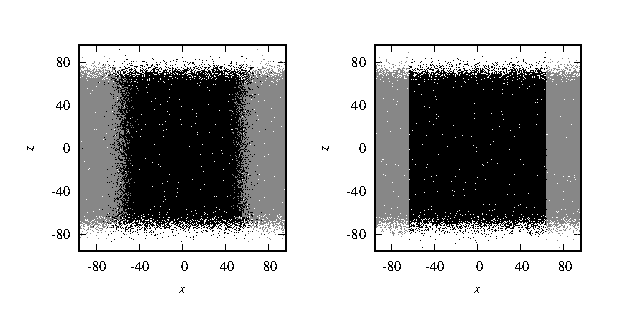
\includegraphics[width = \textwidth]{figures/free_expansion.eps}
  \caption{\label{free_expansion}Free expansion of an ideal gas in the $z$
           direction. The system is periodic along the $xy$ plane. On the left,
           the black dots represent particles that were inside the simulation
           box at the start of the computation, and grey dots represent their
           periodic images. On the right, black dots point out the particles
           inside the simulation box at the end of the computation, while grey
           dots mark the positions of particles in other boxes.}
\end{figure}

\section{Initial conditions}

We have chosen random initial positions, distributed uniformly, for the 
particles; a dangerous choice if we were not dealing with an ideal gas. In many 
systems, particles resist being pushed too close together with great force. As 
you increase the density of particles, you make it more probable for particles 
placed randomly to fall too close to each other. Overlapping particles may feel 
a huge repulsion and shoot off, causing a chain reaction that makes your system 
blow up in the first few steps of a simulation.

A simple solution, apart from reading the initial conditions in from an external 
file, consists in setting particles on the nodes of a crystal lattice and 
letting them reshuffle during the initial stages of the simulation. As an
illustration, include the right header,
\begin{lstlisting}
# include "utils/InitialConditions.cuh"
\end{lstlisting}
and change the inital conditions block to
\begin{lstlisting}
%! codeblock: latticeInitialConditions
  real L = 128;

  %! codeinsert: LJsimulationBox
  {
    auto position
      = particles->getPos(access::location::cpu,
                          access::mode::write);

    auto initial =  initLattice(box.boxSize,
                                numberOfParticles, sc);

    std::copy(initial.begin(), initial.end(), position.begin());
  }
%! codeblockend
\end{lstlisting}
The ``\texttt{sc}'' parameter in \texttt{initLattice} refers to ``simple
cubic''. Other options are face-centred cubic (\texttt{fcc}), body-centred cubic
(\texttt{bcc}), hexagonal close-packed (\texttt{hcp}), diamond structure
(\texttt{dia}) and the two-dimensional triangular (\texttt{tri}) and square
(\texttt{sq}) lattices.

Remember to reset the periodicity of the box in the $z$ direction:
\texttt{periodicityZ = true}.
\begin{comment}
\begin{lstlisting}
%! codeblock: LJsimulationBox
    Box box(make_real3(L, L, L));
    bool periodicityX = true, periodicityY = true,
         periodicityZ = true;
    box.setPeriodicity(periodicityX, periodicityY,
                       periodicityZ);
%! codeblockend
\end{lstlisting}
\end{comment}

Concerning the velocities, the ideal gas example picked random directions and set
the speeds in such a way that you got the energy per particle set among the
parameters. This choice should be fine for our present example, but perhaps you
would later like to experiment imposing an initial sine-shaped velocity profile.
In that event, you could set \texttt{VerletParams.initVelocities} to false and
then write something like this:
\begin{lstlisting}
  {
    auto position
      = particles->getPos(access::location::cpu,
                          access::mode::read);
    auto velocity
      = particles->getVel(access::location::cpu,
                          access::mode::write);

    for(int i = 0; i < numberOfParticles; ++i)
      velocity[i].x
        = sin(2*M_PI*position[i].z/L);
  }
\end{lstlisting}

\section{Interactions}

The final ingredient in our beginner simulations concerns interactions among 
particles. Nothing exciting happens while particles cannot bounce off, repel or 
attract each other. Here we focus on short-range forces, meaning that they fall 
off quicker than the distance between particles squared. If that is the case, 
unless we make the simulation box tiny, particle number $i$ will interact with 
at most one of the periodic copies of particle $j$. The \textit{minimum-image 
convention} states that, when we calculate interactions involving particle 
number $i$, we will neglect all the interactions with periodic images of 
particle number $j$, except perhaps the closest one (see Figure 
\ref{minimum-image_convention}).

A prototypical example of a molecular dynamics simulation involves spheres 
interacting with each other through a Lennard-Jones potential,
\begin{equation*}
  V(r) = 4\epsilon\left(\left(\frac{\sigma}{r}\right)^{12}
                        - \left(\frac{\sigma}{r}\right)^6\right). 
\end{equation*}
The energy $V$ depends on the distance $r$ between the centres of spheres. If 
the particles come closer than $\sigma$, then they feel a strong repulsion. At
greater distances, they attract each other weakly with a force that falls off
as the sixth power of $r$, in accordance with the law for London dispersion
forces. In the right circumstances, particles may stick together, bonding with
an energy equal to $\epsilon$. Systems with Lennard-Jones interactions represent
neutrally-charged swarms of atoms, such as low-temperature argon, and have been
studied in such great detail that they are used extensively for verifying that
code works correctly and for comparing efficiencies.

A very common speed-up trick sets a cut-off radius (usually at
$r = r_{\mathrm{cut}} = 2.5 \sigma$) beyond which $V(r) = 0$. Some researchers
also shift the potential slightly to avoid the discontinuity in $V$ at
$r = r_{\mathrm{cut}}$.

If you want to incorporate the Lennard-Jones interactions, you have to carry out 
the following three steps:
\begin{enumerate}
  \item Specify the functional form of the interaction.
  \item Create an \textit{interactor}.
  \item Add the \textit{interactor} to the \textit{integrator}.
\end{enumerate}

Take each point in turn, beginning with the potential function. To incorporate
it, we add
\begin{lstlisting}
# include "Interactor/Potential/Potential.cuh"
%!
\end{lstlisting}
to our include list at the beginning of the code file. Fortunately, the
Lennard-Jones potential has already been implemented in UAMMD, so we
only need to specify its parameters.
\begin{lstlisting}
%! codeblock: Lennard-JonesPotential
  auto LJPotential = make_shared<Potential::LJ>(sys);
  {
    Potential::LJ::InputPairParameters LJParams;
    LJParams.epsilon = 1.0;
    LJParams.sigma = 1.0;
    LJParams.cutOff = 2.5*LJParams.sigma;
    LJParams.shift = false;
    LJPotential->setPotParameters(0, 0, LJParams);
  }
%! codeblockend
\end{lstlisting}
You should find these parameters self-evident with the exception of the first
two zeros in \texttt{setPotParameters}. These indicate that we are setting the
interaction potential among particles of type 0. If we wished to add, for
example, a different type of interaction between particles of type 0 and 1,
then we would have a similar listing ending in something like
\begin{lstlisting}
    LJPotential->setPotParameters(0, 1, LJParams2);
\end{lstlisting}

Step two mentioned creating an ``interactor''. We will use the
\texttt{PairForces} module.
\begin{lstlisting}
# include "Interactor/PairForces.cuh"
\end{lstlisting}

Taking the point of view of a physicist, think of an interactor as an 
\textit{interaction} that the integrator must take into account to calculate the 
motions. We must provide the algorithm for short-ranged forces with the 
information about the simulation box, so that it can calculate interactions 
using the minimum-image convention, as in the first paragraph in the snippet 
below. We want our interaction to apply to all particles, so we define the 
\texttt{allParticles} group. The new interaction is defined next, using the 
reference to our system (\texttt{particles}), the relevant group 
(\texttt{allparticles}), the system (\texttt{sys}), information about the
simulation box (\texttt{interactionParams}) and, finally, the Lennard-Jones
potential that we defined above (\texttt{LJPotential}).
\begin{lstlisting}
%! codeblock: Lennard-JonesInteraction
  {
    using LJForces = PairForces<Potential::LJ>;
    LJForces::Parameters interactionParams;
    interactionParams.box = box;

    auto allParticles
      = make_shared<ParticleGroup>(particles, sys, "All");

    auto interaction
      = make_shared<LJForces>(particles, allParticles,
                              sys, interactionParams,
                                LJPotential);

    integrator->addInteractor(interaction);
  }
%! codeblockend
\end{lstlisting}
The code block ends with step three: adding the interaction to the integrator
with the \texttt{addIntegrator} method.

With this, we have transformed our ideal gas into a system capable of phase
transitions and interfaces. Remember to change the name of the output file to
something more meaningfull, like ``\texttt{Lennard-Jones.dat}''.
\begin{comment}
\begin{lstlisting}
%! codefile: code/Lennard-Jones.cu
# include "uammd.cuh"
# include "utils/InitialConditions.cuh"
# include "Interactor/Potential/Potential.cuh"
# include "Interactor/NeighbourList/CellList.cuh"
# include "Interactor/PairForces.cuh"
# include "Integrator/VerletNVE.cuh"

using namespace uammd;
using std::make_shared;
using std::endl;

int main(int argc, char *argv[]){

  auto sys = make_shared<System>(argc, argv);

  %! codeinsert: particleData

  %! codeinsert: latticeInitialConditions

  %! codeinsert: VerletParams

  %! codeinsert: Verlet

  %! codeinsert: Lennard-JonesPotential

  %! codeinsert: Lennard-JonesInteraction

  std::string outputFile = "Lennard-Jones.dat";
  std::ofstream out(outputFile);

  int numberOfSteps = 1000;
  int printEverynSteps = 100;

  %! codeinsert: integration

  sys->finish();

  return 0;
}
%! codeend
\end{lstlisting}
\end{comment}

%%%% Figure
%% Compare LJ with ideal gas RDF by deactivating addInteractor line.

\section{Parameter files}

\section{Logging}

\begin{comment}
List of programs written in this chapter:

%! codeblock: codelist
* `minimal.cu`: A minimal UAMMD program that only prints a Hello message and
  then exits.
* `free_expansion.cu`: Ideal gas expanding freely in the vertical direction with
  periodic boundary conditions in the other two directions.
* `Lennard-Jones.cu`: Particles in a periodic box interacting through a
  Lennard-Jones potential.
%! codeblockend
\end{comment}
